\subsubsection{Fit}

Eseguiamo il fit ai minimi quadrati del rate in funzione dell'angolo,
assegnando l'incertezza poissoniana ai rate e \SI{\pm1}{\degree} agli angoli.
Nel caso di collimatore da \SI1{mm} usiamo una funzione proporzionale alla \eqref{eq:rutherford}:
\begin{equation}
	\label{eq:fit1}
	R_1(\theta;B,\theta_0) = \frac {B} {(1-\cos(\theta-\theta_0))^2}.
\end{equation}
Per il collimatore da \SI5{mm} mediamo la \eqref{eq:fit1}
supponendo che il fascio incidente abbia una distribuzione uniforme sul collimatore:
\begin{align*}
	R_5(\theta;B,\theta_0)
	&= \int_{-\ell/2}^{\ell/2} \frac{\de a}{\ell}
	\frac B {(1-\cos(\theta_R(a, \theta-\theta_0)))^2}, \\
	\theta_R(a, \theta)
	&= \tan^{-1} \left( \tan(\theta) - \frac a {L\cos\theta} \right) - \tan^{-1}\frac aD,
\end{align*}
dove $a$ è la coordinata sul collimatore, $\theta_R$ è l'angolo di cui effettivamente viene deviata la traiettoria attraversando il bersaglio,
$L$ e $D$ sono definite in \autoref{sec:forma}, $\ell$ è la larghezza del collimatore.

\begin{figure}
	\hspace{-0.2\textwidth}
	{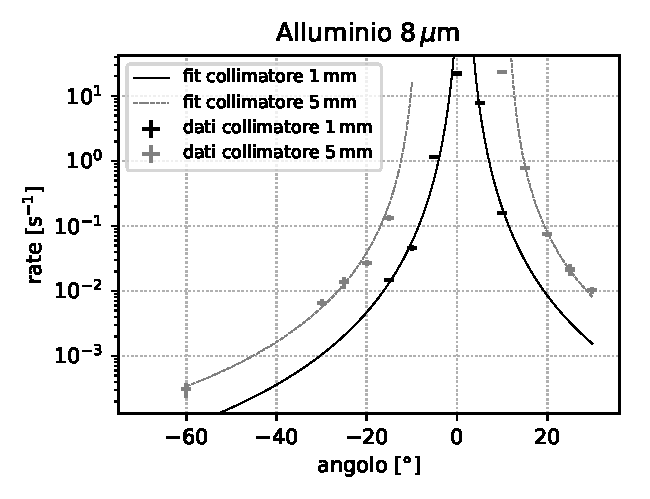
\includegraphics[height=0.5\textwidth]{immagini/all}}
	~
	{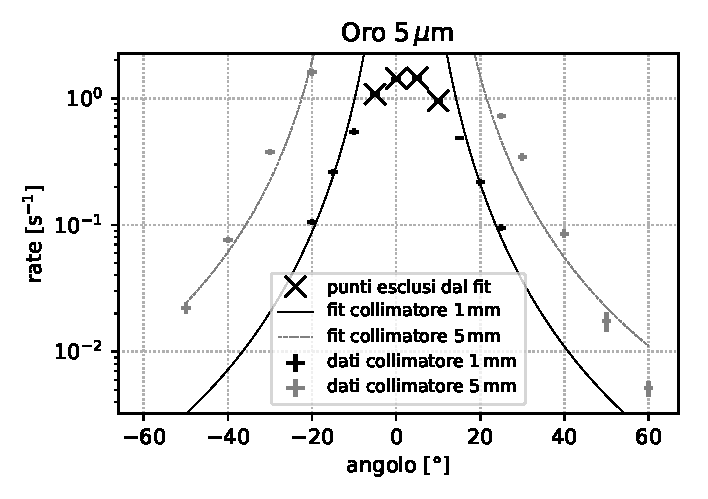
\includegraphics[height=0.5\textwidth]{immagini/oro5}}
	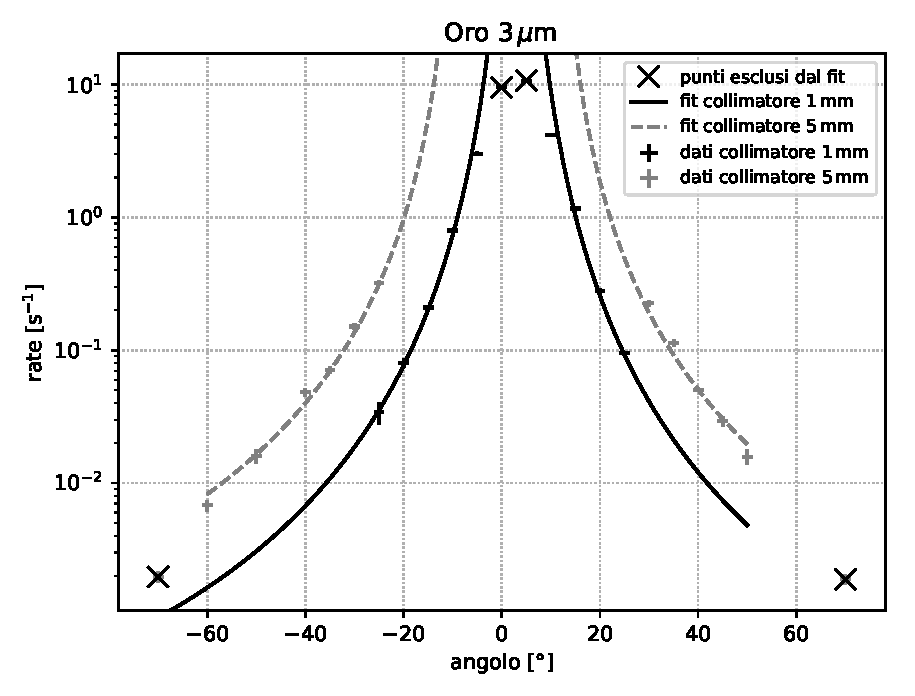
\includegraphics[height=0.5\textwidth]{immagini/oro3}
	\caption{\label{fig:fit}
	cippa}
\end{figure}

\subsubsection{Rapporto delle cariche nucleari}

Comparando i parametri di ampiezza dei fit con l'oro con quello eseguito sull'alluminio, possiamo estrarre lo Z di quest'ultimo. Le ampiezze di fit hanno la forma $$ B=\mathcal{L} \left( \frac {zZ\alpha\hbar c} {2T} \right)^2 = \mathcal{L} A . $$
La nostra luminosità vale $\mathcal{L}=r n_2 l$, in cui $r$ è il rate di particelle incidenti, $n$  è la densità di bersagli e $l$ è lo spessore della targhetta.
Nel nostro caso $n_1$ è uguale per tutte le misure con lo stesso collimatore.   \marginpar{c'è bisogno di precisare perché?}
Da queste considerazioni possiamo trarre lo Z dell'alluminio dalla relazione \eqref{zeta} usando i parametri di fit per i dati con lo stesso collimatore.

\begin{equation}
Z_{\text{al}}=Z_{\text{au}} \sqrt{ \frac{B_{\text{al}}}{B_{\text{au}}} \frac{n_{\text{au}} l_{\text{au}}}{n_{\text{al}} l_{\text{al}}} }
\label{zeta}
\end{equation}

Otteniamo i seguenti risultati:

\begin{align*}
\text{Oro } \SI3{\micro m}&:\\
\text{collimatore } \SI1{mm}&: Z_{\text{al}}=\num{10.4(4)} \\
\text{collimatore } \SI5{mm}&: Z_{\text{al}}=\num{9.2(4)}. \\
\text{Oro } \SI5{\micro m}&:\\
\text{collimatore } \SI1{mm}&: Z_{\text{al}}=\num{13.5(6)} \\
\text{collimatore } \SI5{mm}&: Z_{\text{al}}=\num{70(2)}. \\
\end{align*}

Soltanto una misura è compatibile con lo $Z$ dell'alluminio atteso. Gli altri risultati sono influenzati dallo scattering multiplo all'interno dell'oro, fenomeno praticamente assente nell'alluminio.
L'ultimo risultato è molto lontano dal valore atteso perché lo scattering multiplo influisce pesantemente su una lamina d'oro così spessa e il fatto che il collimatore da \SI5{mm} selezioni più angoli rispetto a quello da \SI1{mm} non fa che peggiorare la situazione.